\chapter{Evaluierung}

\section{Stromverbrauch}

Der Stromverbrauch des Autos ist ein wichtiges Kriterium in den statischen Disziplinen. Um den Stromverbrauch im laufenden Betrieb messen zu können, wird hier ein Versuchsaufbau verwendet welcher der Messung des
Motorstomes ähnelt. Die Schaltung besteht dabei aus einem Shuntwiderstand, einer aktiven Filterschaltung und einem Arduino, welcher die Daten zum NUC weiterleitet. Der Vorteil dieser Methode ist, dass die Daten
unter realen Bedingungen in Echtzeit aufgezeichtet werden können. Abbildung [\ref{fig:Strom}] zeit den Verlauf des Stromes währed folgendem Szenario: Bis ca 25s steht das Auto, sämmtliche Software ist dabei auf 
dem Auto aktiv. Ab 25s beschleunigt das Auto auf $1,3\frac{m}{s}$ und verahrt dort bis ca. Sekunde 57, in welcher es gegen eine Wand fährt. Der grüne Graph stellt dabei den Strom durch den Motor dar, während
der blaue Graph den Gesammtverbrauch des Autos darstellt. Die roten Linien Stellen einen gleitenden Mittelwert aus den letzten 200 Messwerten dar. Gut zu erkenn ist, das der Stromverbrauch des Autos im Stand unter 
10 Watt liegt. Der Mittelwert des Verbrauches im Stand beträgt 7,9 Watt, während das Auto in der dar fahrt knapp 13 Watt an Leistung aufnimmt. Nur während das Auto beschleunigt benötigt es für die Dauer
des Beschleunigungsvorganges mehr Leistung. Fährt das Auto gegen ein Hinderniss, sodas die Räder blockieren befindet sich der Motor im Kurzschlussbetrieb, dabei reduziert sich sein widerstand auf den Ohmschen widerstand
Motors, was zu einem hohen Stromfluss durch den Motor führt. Dauerhaft kann das durch Überhitzung zur Zerstörung des Motors oder der Treiberplatine führen.


\begin{figure}[H]
\centering
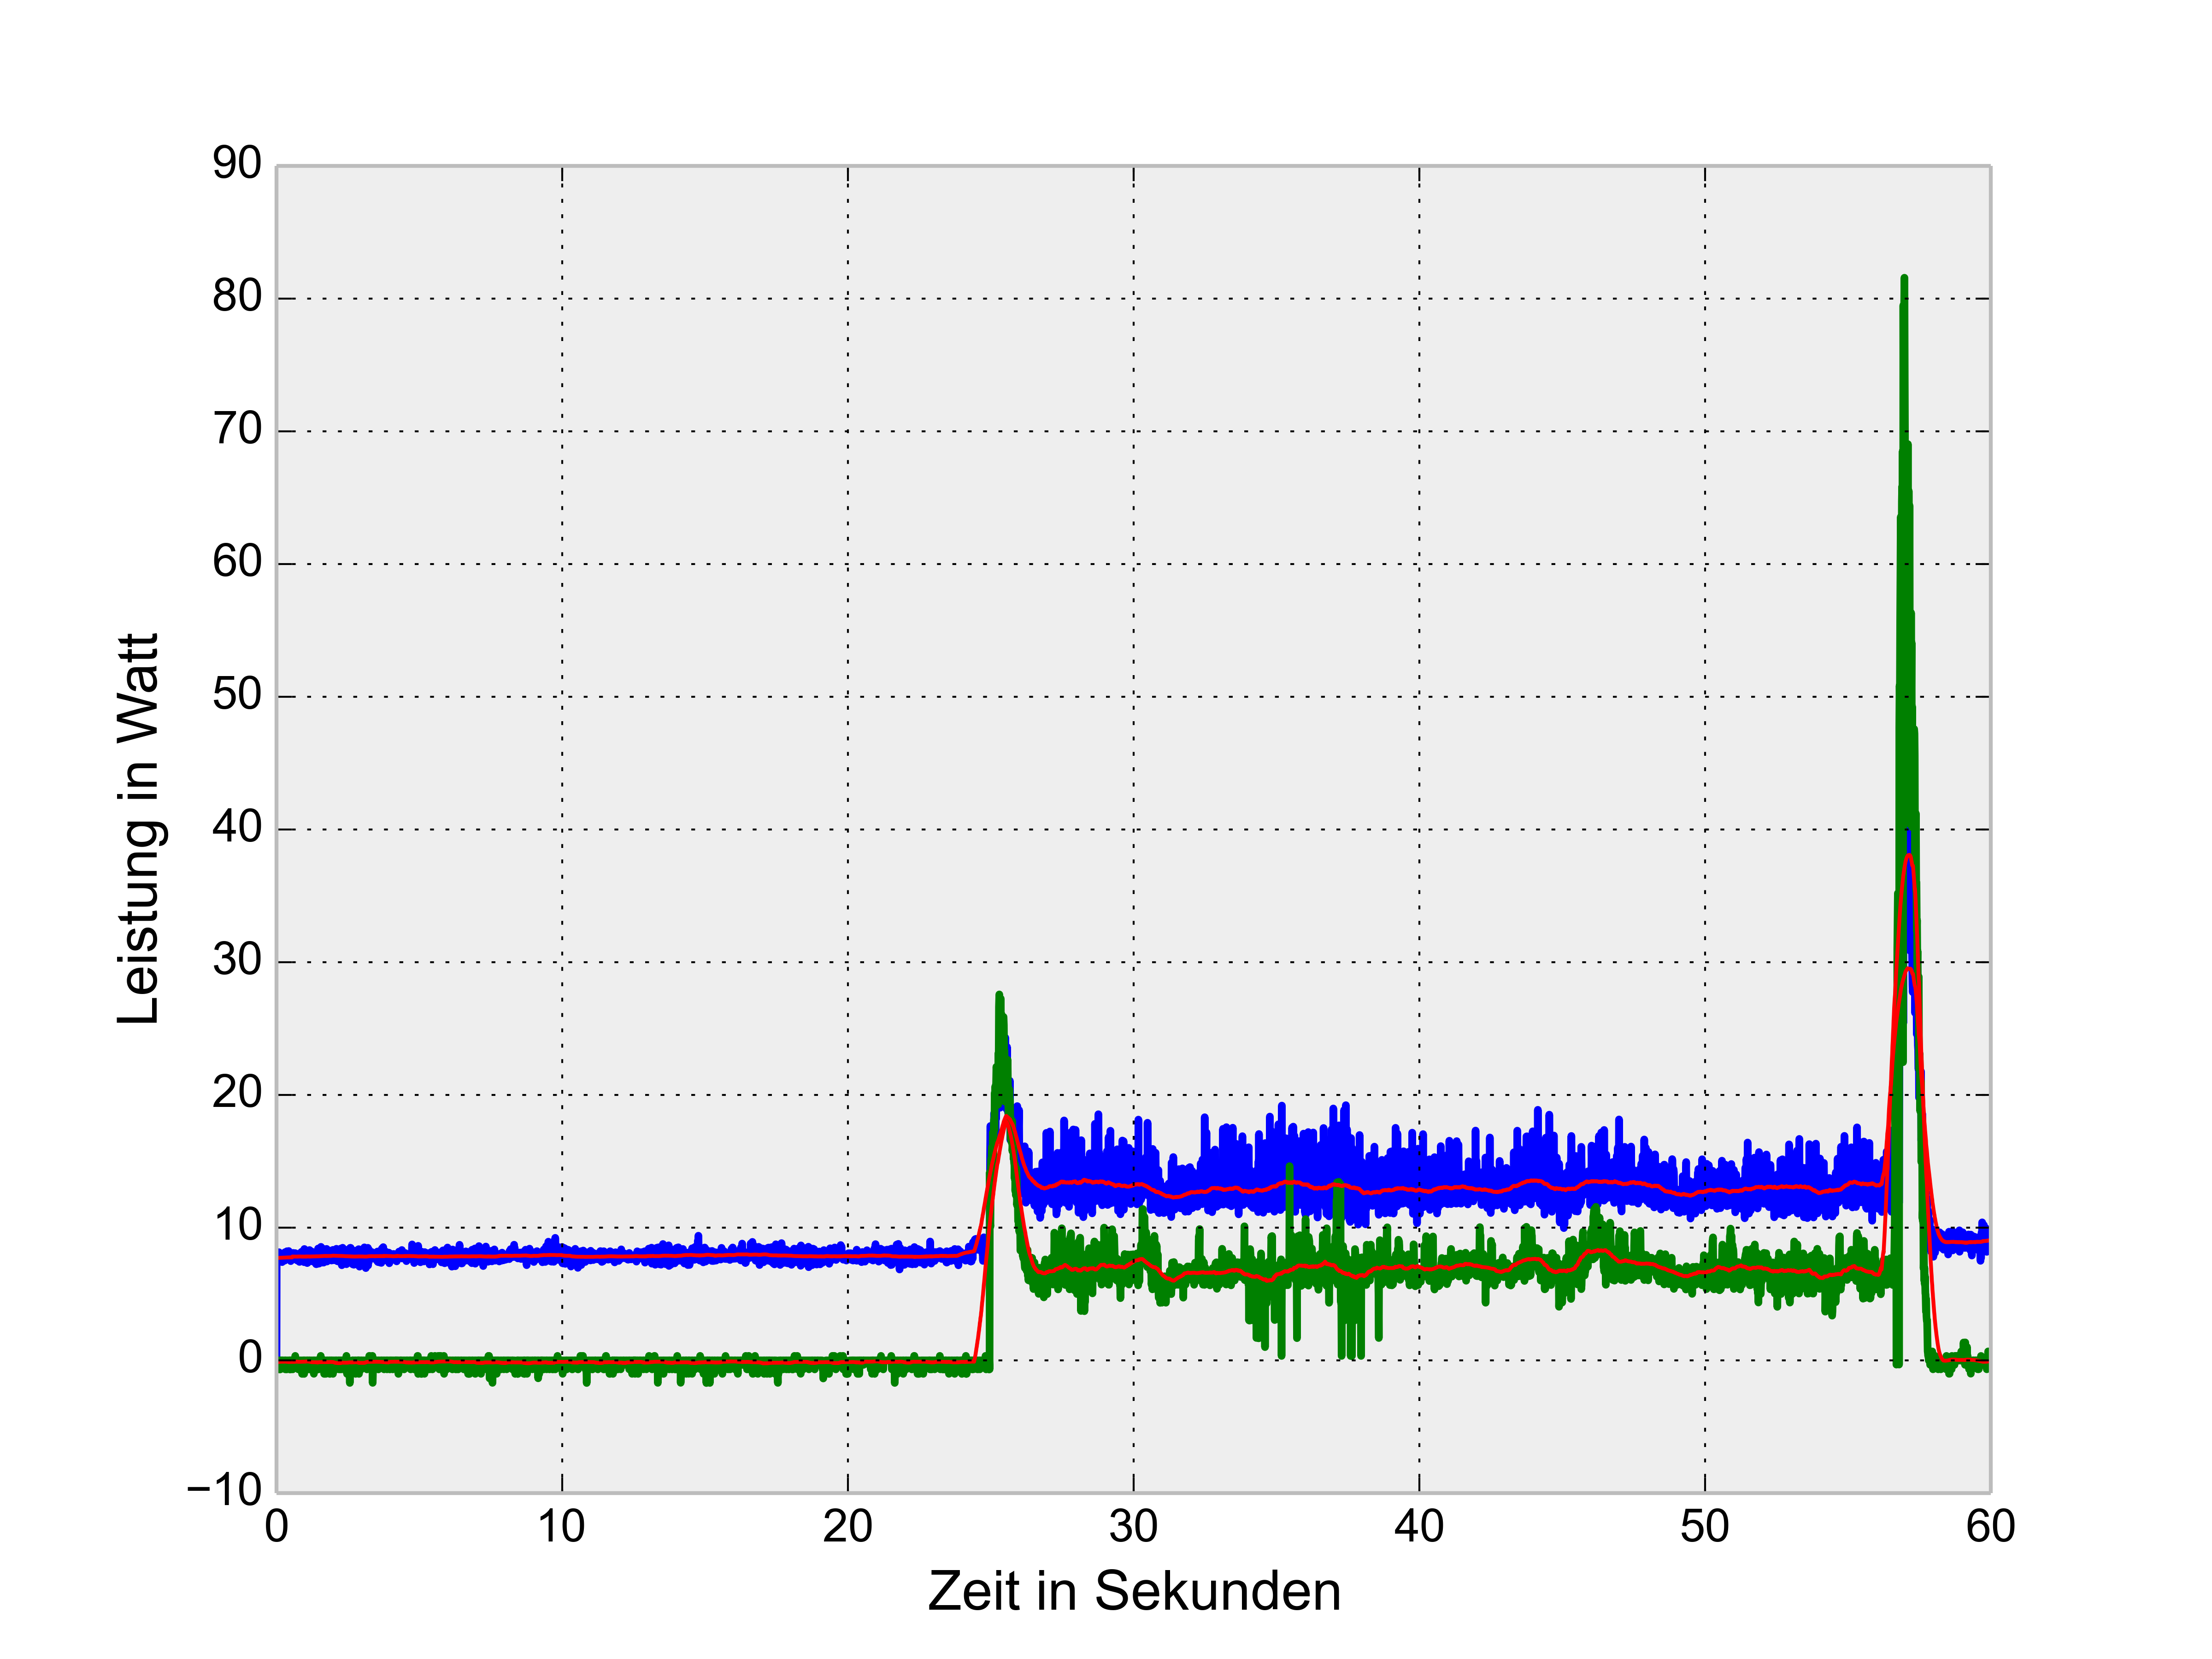
\includegraphics[width=.8\textwidth]{Strom/Power.png}\\
\caption{Salle-Key Tiefpass mit Shunt}%
\label{fig:Strom}
\end{figure}






\section{Infrarotsensoren}

\section{Inertialsensor}

\section{Zeitverhalten der seriellen Verbindung}

Um eine Aussage über das Alter eines Messwertes zu machen. 

\cite{ds-at90can}
adc Wandlung=13Takte
Prescaler=128 bei 16MHz=125000kHz =104uS pro Messung


Bytedauer = 11Bit (1Start+8Daten+2Stopp) 500000Baud --> 22us Bytdauer -> Preamble=5Bytes (4x255+ID) = 110us



\subsection{VoltageCurrent}
25.0319430503
718.591761425


\begin{gnuplot}[terminal=pdf]

  n=70 #number of intervals
  max=872. #max value
  min=596. #min value
  width=(max-min)/n #interval width

  hist(x,width)=width*floor(x/width)+width/2.0

  set xrange [min:max]
  set yrange [0:]

  set offset graph 0.05,0.05,0.05,0.0
  set xtics min,(max-min)/5,max
  set boxwidth width*0.9
  set style fill solid 0.5 #fillstyle
  set tics out nomirror
  set xlabel "x"
  set ylabel "Frequency"
  #count and plot
  plot "MessData/VoltageCurrent.csv" u (hist($1,width)):(1.0) smooth freq w boxes lc rgb"green" notitle
\end{gnuplot}

\subsection{Distance}
28.1616619788
484.734158193


\begin{gnuplot}[terminal=pdf]

  n=70 #number of intervals
  max=673. #max value
  min=359. #min value
  width=(max-min)/n #interval width

  hist(x,width)=width*floor(x/width)+width/2.0

  set xrange [min:max]
  set yrange [0:]

  set offset graph 0.05,0.05,0.05,0.0
  set xtics min,(max-min)/5,max
  set boxwidth width*0.9
  set style fill solid 0.5 #fillstyle
  set tics out nomirror
  set xlabel "x"
  set ylabel "Frequency"
  #count and plot
  plot "MessData/Distance.csv" u (hist($1,width)):(1.0) smooth freq w boxes lc rgb"green" notitle
\end{gnuplot}


\subsection{Infrared}
35.0709303606
696.91743058



\begin{gnuplot}[terminal=pdf]

  n=70 #number of intervals
  max=825. #max value
  min=586. #min value
  width=(max-min)/n #interval width

  hist(x,width)=width*floor(x/width)+width/2.0

  set xrange [min:max]
  set yrange [0:]

  set offset graph 0.05,0.05,0.05,0.0
  set xtics min,(max-min)/5,max
  set boxwidth width*0.9
  set style fill solid 0.5 #fillstyle
  set tics out nomirror
  set xlabel "x"
  set ylabel "Frequency"
  #count and plot
  plot "MessData/Infrared.csv" u (hist($1,width)):(1.0) smooth freq w boxes lc rgb"green" notitle
\end{gnuplot}


\subsection{uCTime}
31.2060346589
477.761007865



\begin{gnuplot}[terminal=pdf]

  n=70 #number of intervals
  max=685. #max value
  min=366. #min value
  width=(max-min)/n #interval width

  hist(x,width)=width*floor(x/width)+width/2.0

  set xrange [min:max]
  set yrange [0:]

  set offset graph 0.05,0.05,0.05,0.0
  set xtics min,(max-min)/5,max
  set boxwidth width*0.9
  set style fill solid 0.5 #fillstyle
  set tics out nomirror
  set xlabel "x"
  set ylabel "Frequency"
  #count and plot
  plot "MessData/ucTime.csv" u (hist($1,width)):(1.0) smooth freq w boxes lc rgb"green" notitle
\end{gnuplot}

\subsection{Motor}
38.0093527069
391.111706657


\begin{gnuplot}[terminal=pdf]

  n=70 #number of intervals
  max=534. #max value
  min=287. #min value
  width=(max-min)/n #interval width

  hist(x,width)=width*floor(x/width)+width/2.0

  set xrange [min:max]
  set yrange [0:]

  set offset graph 0.05,0.05,0.05,0.0
  set xtics min,(max-min)/5,max
  set boxwidth width*0.9
  set style fill solid 0.5 #fillstyle
  set tics out nomirror
  set xlabel "x"
  set ylabel "Frequency"
  #count and plot
  plot "MessData/motor.csv" u (hist($1,width)):(1.0) smooth freq w boxes lc rgb"green" notitle
\end{gnuplot}




\subsection{IMU}
40.8272894054
3425.96398337


\begin{gnuplot}[terminal=pdf]

  n=70 #number of intervals
  max=3605. #max value
  min=3312. #min value
  width=(max-min)/n #interval width

  hist(x,width)=width*floor(x/width)+width/2.0

  set xrange [min:max]
  set yrange [0:]

  set offset graph 0.05,0.05,0.05,0.0
  set xtics min,(max-min)/5,max
  set boxwidth width*0.9
  set style fill solid 0.5 #fillstyle
  set tics out nomirror
  set xlabel "x"
  set ylabel "Frequency"
  #count and plot
  plot "MessData/imu.csv" u (hist($1,width)):(1.0) smooth freq w boxes lc rgb"green" notitle
\end{gnuplot}


\subsection{Gesammt}
142.365993405
6195.08004809


\begin{gnuplot}[terminal=pdf]

  n=70 #number of intervals
  max=6522. #max value
  min=5574. #min value
  width=(max-min)/n #interval width

  hist(x,width)=width*floor(x/width)+width/2.0

  set xrange [min:max]
  set yrange [0:]

  set offset graph 0.05,0.05,0.05,0.0
  set xtics min,(max-min)/5,max
  set boxwidth width*0.9
  set style fill solid 0.5 #fillstyle
  set tics out nomirror
  set xlabel "x"
  set ylabel "Frequency"
  #count and plot
  plot "MessData/gesammt.csv" u (hist($1,width)):(1.0) smooth freq w boxes lc rgb"green" notitle
\end{gnuplot}